\documentclass{article}
\usepackage[polish]{babel}
\usepackage[OT4]{fontenc}
\usepackage[utf8]{inputenc}
\usepackage{hyperref}
\usepackage{graphicx}
\usepackage{amsmath}
\title{\textbf{Praca projektowa z przedmiotu Sztuczna Inteligencja}}
\author{Bartłomiej Czajka 169522 2 EF-DI P1}
\date{Rzeszów, 2023}
\begin{document}
\maketitle
\pagebreak



\tableofcontents{}
\section{Opis projektu}
\subsection{Założenia projektowe}
Celem projektu jest realizacja sieci neuronowej uczonej za pomocą algorytmu sieci głębokiej, klasyfikującej chorobę Parkinsona oraz zbadanie wpływu parametrów sieci na proces uczenia.
Projekt został zrealizowany w języku Python z wykorzystaniem biblioteki PyTorch.
\subsection{Zestaw danych}
Zestaw danych uczących został pobrany ze strony \href{http://archive.ics.uci.edu/ml/datasets/Parkinsons}{http://archive.ics.uci.edu/ml/datasets/Parkinsons}.
Zawiera on 197 instancji, 23 cechy oraz 2 klasy. Dane są nieuporządkowane, nie ma danych nieokreślonych.
Dokładniejszy opis cech zestawu:
\begin{itemize}
    \item name - Nazwa badanego pacjenta w ASCII i numer nagrania.
    \item MDVP:Fo(Hz) - Średnia częstotliwość podstawowa głosu.
    \item MDVP:Fhi(Hz) - Maksymalna częstotliwość podstawowa głosu.
    \item MDVP:Flo(Hz) - Minimalna częstotliwość podstawowa głosu.
    \item MDVP:Jitter(\%), MDVP:Jitter(Abs), MDVP:RAP, MDVP:PPQ, Jitter:DDP - Kilka miar zmienności częstotliwości podstawowej.
    \item MDVP:Shimmer, MDVP:Shimmer(dB), Shimmer:APQ3, Shimmer:APQ5, MDVP:APQ, Shimmer:DDA - Kilka miar zmienności amplitudy.
    \item NHR, HNR - Dwie miary stosunku szumu do składowych tonalnych w głosie.
    \item status - Stan zdrowia badanego (jeden) - chory na Parkinsona, (zero) - zdrowy.
    \item RPDE, D2 - Dwie miary złożoności dynamicznej nieliniowej.
    \item DFA - Wykładnik skalowania fraktalnego sygnału.
    \item spread1, spread2, PPE - Trzy nieliniowe miary zmienności częstotliwości podstawowej.
\end{itemize}
\subsection{Przygotowanie danych}
Sieć ma za zadanie sklasyfikować czy pacjent cierpi na chorobę Parkinsona. Wartość '1' oznacza osobę cierpiącą na chorobę Parkinsona, natomiast '0' oznacza osobę zdrową.
Dane zostały uporządkowane i znormalizowane.
Normalizacja została wykonana dla każdej obserwacji przy użyciu wzoru:
\[
    x_{\text{norm}} = \frac{{x_{\text{norm\_max}} - x_{\text{norm\_min}}}}{{x_{\text{max}} - x_{\text{min}}}} \cdot (x - x_{\text{min}}) + x_{\text{norm\_min}}
\]

gdzie:
\begin{itemize}
    \item $x_{min}$ - to wektor zawierający minimalne wartości dla każdej obserwacji.
    \item $x_{max}$ - to wektor zawierający maksymalne wartości dla każdej obserwacji.
    \item $x_{norm\_min}$ - to wartość minimalna po normalizacji (-1).
    \item $x_{norm\_max}$ - to wartość maksymalna po normalizacji (1).
    \item $x_{norm}$ - to macierz zawierająca znormalizowane dane.
    \item $x$ - to macierz zawierająca dane wejściowe.
\end{itemize}
\section{Zagadnienia teoretyczne}
\subsection{Wstęp do sieci neuronowych}

Sieci neuronowe to jedno z najbardziej fascynujących paradygmatów programowania, jakie kiedykolwiek powstały.
W tradycyjnym podejściu do programowania komputerowi nakazujemy, co ma zrobić, dzieląc duże problemy na wiele mniejszych, precyzyjnie określonych zadań, które komputer może łatwo realizować.
W przypadku sieci neuronowych nie instruujemy komputera, jak ma rozwiązać nasz problem.
Zamiast tego, sieć neuronowa uczy się na podstawie obserwacji danych, tworząc własne rozwiązanie dla danego problemu.
Jednakże do roku 2006 nie mieliśmy sposobu na efektywne szkolenie sieci neuronowych, które przewyższałyby bardziej tradycyjne podejścia.
To, co zmieniło się w 2006 roku, to odkrycie technik uczenia w tzw. głębokich sieciach neuronowych, znane teraz jako głębokie uczenie.
Od tego czasu, głębokie uczenie jest stale rozwijane i obecnie osiąga wybitne wyniki w wielu ważnych dziedzinach, takich jak widzenie komputerowe, rozpoznawanie mowy czy też przetwarzanie języka naturalnego.
Są one szeroko wdrażane przez takie firmy jak Google, Microsoft i Facebook.


\subsection{Historia sieci neuronowych}


Historia sztucznych neuronów sięga lat 40. XX wieku, kiedy Warren McCulloch, neurobiolog, i Walter Pitts, logik, zaproponowali modelowanie biologicznego działania organicznego neuronu w ramach pierwszego sztucznego neuronu.
Ich celem było pokazanie, jak proste jednostki mogą replikować funkcje logiczne.


Zainspirowany publikacją Warrena McCullocha i Waltera Pittsa, Frank Rosenblatt pracował w latach 50. nad Perceptronem: pojedynczą warstwą neuronów zdolną do klasyfikacji obrazów o wielkości kilkuset pikseli.
Można to uznać za pierwszego przodka współczesnych sieci neuronowych.
Geniusz Rosenblatta polegał na zaimplementowaniu algorytmu trenowania neuronów na podstawie zbioru danych.
Rosenblatt zainspirował się pracami kanadyjskiego psychologa Donalda Hebba, który w swojej książce Organization of Behavior z 1949 roku teoretyzował, że połączenia między neuronami (organicznymi) są wzmacniane w miarę ich używania (zostanie to potwierdzone dopiero w latach 60-tych).
Pomysł Rosenblatta polegał na powieleniu tego za pomocą jego Perceptronu.
New York Times donosił, że Rosenblatt prorokował, iż Perceptrony w przyszłości będą w stanie "rozpoznawać ludzi i wołać ich imiona", "błyskawicznie tłumaczyć mowę w jednym języku na mowę lub pismo w innym języku", "być wystrzeliwane na planety jako mechaniczni eksploratorzy kosmosu", ale także "reprodukować się" i być samoświadome.

Niestety, ze względu na algorytm uczenia, Perceptron był ograniczony do pojedynczej warstwy neuronów.
Pomimo dużego zainteresowania tymi wczesnymi osiągnięciami, profesorowie MIT Marvin Minsky i Seymour Papert opublikowali w 1969 roku książkę (Perceptrons: An introduction to computational geometry ) pokazującą, że Perceptron miał ograniczone możliwości.
Spowodowało to pierwszą "zimę sieci neuronowych" do połowy lat 80.

Paul Werbos, w swojej pracy doktorskiej z 1974 roku, jako pierwszy zaproponował wykorzystanie backpropagacji do optymalizacji sieci neuronowych.
Jednak, jako że byliśmy w pierwszej zimie sieci neuronowych, jego praca przeszła niezauważona przez środowisko naukowe.
Dopiero później, za sprawą pracy Rumelharta et al. (1986), backpropagacja została spopularyzowana jako technika treningowa dla sieci neuronowych.
Uzbrojeni w backpropagację, badacze mogli teraz używać sieci neuronowych w wielu przypadkach użycia.
W szczególności sieci neuronowe zostały wykorzystane do rozpoznawania pisma ręcznego na podstawie techniki zaproponowanej w 1989 roku przez Yanna LeCuna.
Jego model został z powodzeniem zaimplementowany, kończąc na odczytywaniu cyfr napisanych ręcznie w około 10 do 20\% wszystkich czeków przetwarzanych w USA.
Niemniej jednak wkrótce pojawił się nowy problem, powodujący, że uczenie stawało się powolne i niestabilne.

W miarę jak sieci neuronowe stawały się coraz głębsze (z większą liczbą warstw), wsteczna propagacja stawała się wolniejsza z powodu problemu znikających gradientów.
Mówiąc prosto, algorytm wstecznej propagacji wymaga użycia pochodnych (zboczy) funkcji aktywacji.
W tamtych czasach, funkcje aktywacji były głównie sigmoidalne i tanh.
Gdy układasz wiele warstw, zejście gradientowe staje się coraz wolniejsze dla głębszych warstw, co powoduje wykładniczo powolną optymalizację.

Na początku lat 2010, wiele badań zalecało użycie określonej funkcji aktywacji (ReLu) w neuronach do przekazywania informacji. To, wraz z lepszymi algorytmami optymalizacji (takimi jak ADAM), pomogło w efektywnym trenowaniu głębszych sieci neuronowych.


W ostatnich latach dokonano znaczącego postępu w dziedzinie sztucznej inteligencji.
Sztuczna inteligencja taka jak AlphaGo i GPT-3 wykazały zdolność do osiągania wyjątkowych wyników w dziedzinach gier planszowych i generowania tekstów. Jednak to tylko początek. W przyszłości możemy spodziewać się dalszego rozwoju sztucznej inteligencji, która będzie coraz bardziej zaawansowana i wszechstronna.
Sztuczna inteligencja ma potencjał do rewolucjonizowania różnych dziedzin, takich jak medycyna, przemysł, transport czy badania naukowe.
Jej zdolność do szybkiego uczenia się, analizowania ogromnych ilości danych i podejmowania złożonych decyzji otwiera nowe możliwości i perspektywy.
\subsection{Matematyczny opis sztucznego neuronu}
Podstawowym elementem budującym strukturę sieci neuronowej jest neuron. Jest to element, który przetwarza informacje.
W pewnym, uproszczonym stopniu jest wzorowany na funkcjonowaniu biologicznej komórki nerwowej.
Struktura neuronu zawiera wiele wejść oraz jedno wyjście.
Jednym z najważniejszych składników neuronu są wagi, których wartości decydują o zachowaniu neuronu. Są one zazwyczaj ustalane w trakcie procesu uczenia.

\begin{figure}[h]
    \centering
    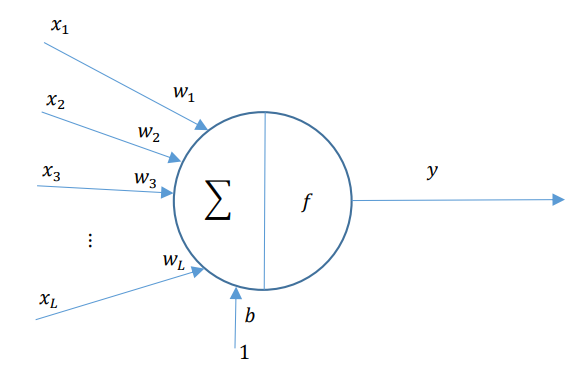
\includegraphics[width=0.7\textwidth]{model_neuronu.png}
    \caption{Model neuronu [4]}
    \label{fig:zdjecie}
\end{figure}
Każdy pojedynczy neuron przyjmuje sygnały wejściowe, które są następnie przetwarzane.
Każde wejście ma przypisany współczynnik wagowy, który określa, jak bardzo wpływa ono na wynik neuronu.
Dodatkowo, neuron posiada "bias", czyli wartość stałą, która jest taka sama dla wszystkich neuronów w danej warstwie.
Wszystkie te informacje są sumowane, gdzie jest obliczane łączne pobudzenie neuronu.
Następnie wartość pobudzenia przechodzi przez funkcję aktywacji, która określa sygnał wyjściowy neuronu, który jest określony wzorem:
\[
    y = \sum_{j=1}^{L} f(w_{j} x_{j} + b)
\]

gdzie:
\begin{itemize}
    \item $j$ -- indeks, który przyjmuje wartości od 1 do $L$,
    \item $y$ -- wyjście neuronu,
    \item $w_{j}$ -- współczynnik wagowy przypisany do $j$-tego wejścia,
    \item $x_{j}$ -- $j$-ty sygnał wejściowy,
    \item $b$ -- bias [2].
\end{itemize}

\subsection{Sieć głęboka}
\section{Realizacja sieci neuronowej}
\subsection{Opis skryptu}
\section{Eksperymenty}
\subsection{Eksperyment 1}
\subsection{Eksperyment 2}
\subsection{Eksperyment 3}
\section{Wnioski}
\begin{thebibliography}{9}
    \bibitem{Nielsen}
    Michael Nielsen,
    \emph{Neural Networks and Deep Learning}.
    Determination Press,
    2015.
    \bibitem{TadeusiewiczSzaleniec}
    Ryszard Tadeusiewicz, Maciej Szaleniec,
    \emph{Leksykon sieci neuronowych}.
    Wrocław,
    2015.
    \bibitem{vandeput}
    Nicolas Vandeput,
    \href{https://medium.com/analytics-vidhya/a-brief-history-of-neural-networks-c234639a43f1}{\emph{A Brief History Of Neural Networks}},
    [dostęp: 15.05.2023].
    \bibitem{zajdel}
    Zajdel R.,
    \emph{Ćwiczenie 4 Model Neuronu},
    Rzeszów,
    KIiA, PRz.
\end{thebibliography}
\end{document}